\chapter{\IfLanguageName{dutch}{Stand van zaken}{State of the art}}%
\label{ch:stand-van-zaken}

In dit hoofdstuk van de bachelorproef zullen we dieper ingaan op het concept van een microservices-architectuur. Dit zal gebeuren aan de hand van een relevante literatuurstudie. Allereerst zal uitgelegd worden wat een monolithische architectuur is en wat typerend is aan deze stijl van software ontwikkeling. Daarna wordt uitgelegd wat een microservices-architectuur is en hoe deze architectuur verschilt van de klassieke, monolithische aanpak. Tot slot worden enkele relevante termen uitgebreider behandelt die de werking en structuur van microservices definiëren. Op basis van de informatie uit dit hoofdstuk zal duidelijk worden wat er allemaal komt kijken tijdens het ontwerpen van een proof-of-concept (PoC) in een later deel van de bachelorproef.

\section{Wat is een monolithische architectuur?}

De monolithische architectuur is door de jaren heen een succesvolle keuze geweest voor softwareontwikkelaars \autocite{Gos2020}. Bij deze aanpak van software ontwikkeling bestaat een applicatie uit verscheidene componenten. Voorbeelden van componenten zijn authenticatie en authorizatie, productbeheer, klantenbeheer enz. Deze componenten bevinden zich in een monolithische architectuur dan in één en hetzelfde programma.

\begin{figure}[H]
  \centering
  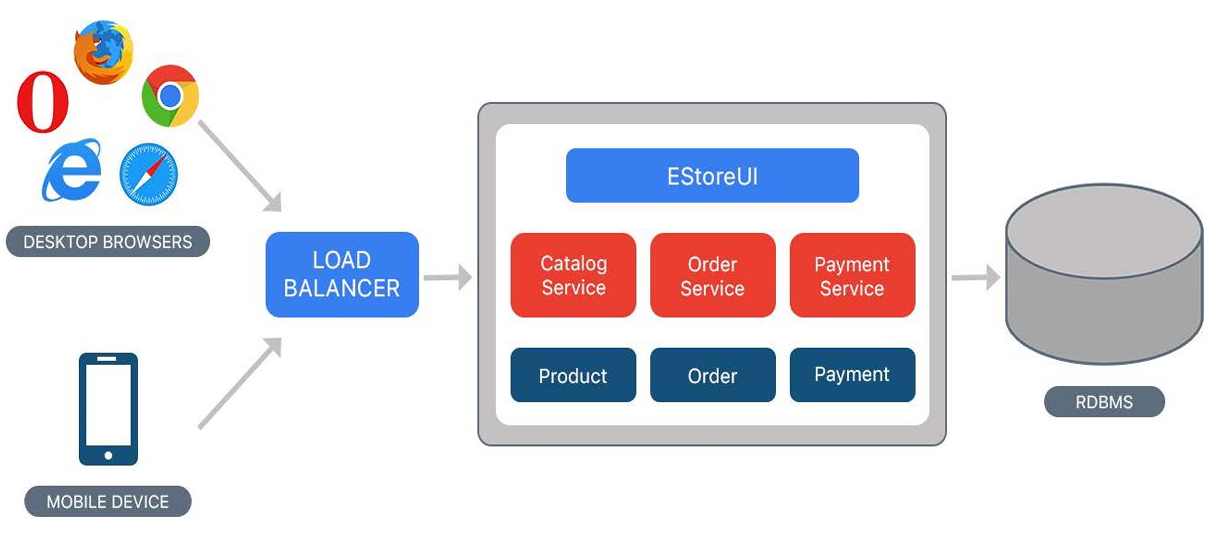
\includegraphics[width=0.85\textwidth]{MonolithischeArchitectuur.png}
  \caption[Voorstelling van een monolitische architectuur]{\label{fig:monolithische architectuur}Voorbeeld van een monolithische architectuur. Deze afbeelding toont de architectuur van een applicatie die de bedrijfslogica voor een e-commerce demonstreert \autocite{Gos2020}.}
\end{figure}

De bovenstaande afbeelding (Figuur \ref{fig:monolithische architectuur}) verduidelijkt de interne structuur van een monolithische applicatie. In deze representatie zien we een EStoreUI component die fungeert als de grafische interface waarmee gebruikers kunnen interageren met de applicatie. Daaronder zijn 3 services gedefiniëerd, namelijk de Catalog Service, Order Service en Payment Service. Elk van deze 3 services is verantwoordelijk voor het respectievelijke bedrijfsproces. Tot slot zijn alle services verbonden met eenzelfde relationele database (RDBMS). Deze verschillende componenten bevinden zich in een monolithische architectuur dan ook binnen dezelfde applicatie.\newline

Een kenmerkend aspect van een monolithische applicatie is de gelaagde structuur, waarbij de grafische interface bovenop verschillende services is opgebouwd en waar er slechts 1 databank is die gedeeld wordt door alle services \autocite{Velepucha2023}. Deze architectuur staat ook beter bekend als het 3-lagenmodel, waarbij de opbouw van een applicatie wordt opgedeeld in diverse lagen. De volgende lagen kunnen geïdentificeerd worden:

\begin{itemize}
	\item \textbf{Presentatielaag}: binnen deze laag vinden we de code die het mogelijk maakt voor gebruikers om met de applicatie te interageren.
	\item \textbf{Business laag}: deze laag is specifiek ontworpen met het oog op het implementeren van bedrijfsfunctionaliteit en validatie.
	\item \textbf{Datalaag}: hierin worden alle interacties met de dataopslag gedefinieerd alsook de interacties met externe services die nodig zijn voor de applicatie.
\end{itemize}

De monolithische architectuur brengt een aantal voordelen met zich mee, zoals eenvoudige implementatie en gemakkelijke testbaarheid \autocite{Li2022}. Toch zijn er ook een aantal mindere aspecten aan deze software architectuur, voornamelijk wanneer de applicatie dient te groeien. Naarmate bedrijven groeien en hun software uitbreiden, kan de toenemende grote van de codebase leiden tot verschillende problemen \autocite{Wei2025}. Wijzigingen in de functionaliteiten of bugfixes kunnen bijvoorbeeld onverwachte gevolgen hebben voor de gehele applicatie. Daarnaast heeft de sterke opkomst van cloud computing de voordelen van een monolithische architectuur opmerkelijk verminderd. Cloud-gebaseerde oplossingen vereisen vaak schaalbaarheid en flexibiliteit. Deze 2 factoren sluiten minder goed aan bij de klassieke, monolithische applicatie. Volgens \textcite{Wei2025} heeft deze evolutie dan ook geleid tot een toenemende interesse in microservices.

\section{Wat is een microservices-architectuur?}

Succesvolle softwaresystemen groeien in de loop van de tijd vaak in omvang en complexiteit \autocite{Abgaz2023}. Dit door de toevoeging van verschillende functionaliteiten, wat kan resulteren in sterk gekoppelde, maar toch minder samenhangende componenten. Als gevolg hiervan hebben monolithische applicaties vaak beperkingen op het gebied van schaalbaarheid, onderhoud en prestaties. In de huidige bedrijfsomgevingen is de nood om schaalbare applicaties te ontwikkelen essentieel, wegens de opkomst van nieuwe technologieën en de vraag om zowel menselijke als technologische middelen te optimaliseren \autocite{Nayim2023}.\newline

Een van de allereersten die een definitie voor microservices gaven waren \textcite{Lewis2014}. Zij beschreven in hun blogpost de microservices-architectuur als een software architectuur waarbij één enkele applicatie bestaat uit verschillende, kleinere services. Deze kleinere services kunnen onafhankelijk van elkaar werken en communiceren met elkaar door gebruik te maken van bijvoorbeeld Hypertext Transfer Protocol (HTTP) of een Application Programming Interface (API). Wanneer we dan kijken naar een recentere beschrijving van dit concept, dan benadrukken \textcite{Velepucha2023} dat de microservices-architectuur een vorm is van een \hyperref[sec:distributed systems]{gedistribueerd systeem} waarin services onafhankelijk kunnen werken. Daarnaast voegen ze er nog aan toe dat elke service binnen deze architectuur een specifieke bedrijfsfunctionaliteit dient te vervullen.

\begin{figure}[H]
	\centering
	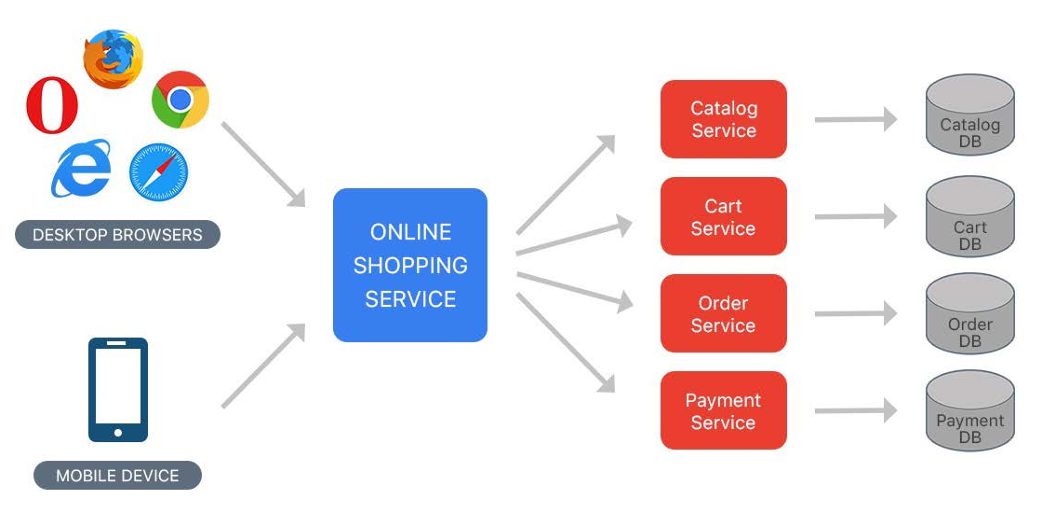
\includegraphics[width=0.75\textwidth]{MicroservicesArchitectuur.png}
	\caption[Voorstelling van een microservices architectuur]{\label{fig:microservices architectuur}Voorbeeld van een microservices architectuur. Deze afbeelding toont een vereenvoudigde representatie van een applicatie met microservices \autocite{Gos2020}.}
\end{figure}

Hierboven wordt de kern van de microservices-architectuur weergegeven. Eerder in dit hoofdstuk zagen we een gelijkaardige representatie, maar dan voor een monolithische architectuur. Daarin benadrukten we dat alle services binnen eenzelfde applicatie behoorden. Hier zien we nu dat alle 4 de services los van elkaar staan en dat ze toegankelijk zijn via één dirigerende service. Een ander opvallend aspect van deze software architectuur, die bij de bovenstaande definities van microservices niet vermeld werd, is dat elke service zijn eigen databank heeft.\newline

De belangrijkste principes van deze architectuur zijn \autocite{Blinowski2022}:

\begin{itemize}
	\item \textbf{Één verantwoordelijkheid per service} - Volgens de SOLID-principes\footnote{Dit is een TEST!} moet elke service ter allen tijde slechts en alleen één verantwoordelijkheid hebben. Nooit mogen twee of meerdere services eenzelfde verantwoordelijkheid delen.
	\item \textbf{Microservices zijn autonoom} - Elke microservice is volledig verantwoordelijk voor het uitvoeren van een specifieke bedrijfsfunctionaliteit. Hierdoor bevatten ze alle benodigde afhankelijkheden, zoals bibliotheken.
	\item \textbf{Services zijn volwaardige componenten} - Eindpunten worden ter beschikking gesteld als API's en verbergen de interne implementatiedetails. De logica, architectuur en gebruikte technologieën blijven volledig verborgen achter de API.
\end{itemize}

\subsection{Karakteristieken van microservices}

\section{Relevante termen}

\subsection{Distributed Systems}
\label{sec:distributed systems}

\subsection{Service-Oriented Architecture}

\subsection{Enterprise Service Bus}

\subsection{Polyglot persistence}

\subsection{Docker}

\subsection{Kubernetes}

% Tip: Begin elk hoofdstuk met een paragraaf inleiding die beschrijft hoe
% dit hoofdstuk past binnen het geheel van de bachelorproef. Geef in het
% bijzonder aan wat de link is met het vorige en volgende hoofdstuk.

% Pas na deze inleidende paragraaf komt de eerste sectiehoofding.

%Dit hoofdstuk bevat je literatuurstudie. De inhoud gaat verder op de inleiding, maar zal het onderwerp van de bachelorproef *diepgaand* uitspitten. De %bedoeling is dat de lezer na lezing van dit hoofdstuk helemaal op de hoogte is van de huidige stand van zaken (state-of-the-art) in het %onderzoeksdomein. Iemand die niet vertrouwd is met het onderwerp, weet nu voldoende om de rest van het verhaal te kunnen volgen, zonder dat die er nog %andere informatie moet over opzoeken \autocite{Pollefliet2011}.

%Je verwijst bij elke bewering die je doet, vakterm die je introduceert, enz.\ naar je bronnen. In \LaTeX{} kan dat met het commando %\texttt{$\backslash${textcite\{\}}} of \texttt{$\backslash${autocite\{\}}}. Als argument van het commando geef je de ``sleutel'' van een ``record'' in %een bibliografische databank in het Bib\LaTeX{}-formaat (een tekstbestand). Als je expliciet naar de auteur verwijst in de zin (narratieve %referentie), gebruik je \texttt{$\backslash${}textcite\{\}}. Soms is de auteursnaam niet expliciet een onderdeel van de zin, dan gebruik je %\texttt{$\backslash${}autocite\{\}} (referentie tussen haakjes). Dit gebruik je bv.~bij een citaat, of om in het bijschrift van een overgenomen %afbeelding, broncode, tabel, enz. te verwijzen naar de bron. In de volgende paragraaf een voorbeeld van elk.

%\textcite{Knuth1998} schreef een van de standaardwerken over sorteer- en zoekalgoritmen. Experten zijn het erover eens dat cloud computing een %interessante opportuniteit vormen, zowel voor gebruikers als voor dienstverleners op vlak van informatietechnologie~\autocite{Creeger2009}.

%Let er ook op: het \texttt{cite}-commando voor de punt, dus binnen de zin. Je verwijst meteen naar een bron in de eerste zin die erop gebaseerd is, %dus niet pas op het einde van een paragraaf.

%\begin{figure}
%  \centering
%  
\includegraphics[width=0.8\textwidth]{grail.jpg}
%  \caption[Voorbeeld figuur.]{\label{fig:grail}Voorbeeld van invoegen van een figuur. Zorg altijd voor een uitgebreid bijschrift dat de figuur %volledig beschrijft zonder in de tekst te moeten gaan zoeken. Vergeet ook je bronvermelding niet!}
%\end{figure}

%\begin{listing}
%  \begin{minted}{python}
%    import pandas as pd
%    import seaborn as sns
%
%    penguins = sns.load_dataset('penguins')
%    sns.relplot(data=penguins, x="flipper_length_mm", y="bill_length_mm", hue="species")
%  \end{minted}
%  \caption[Voorbeeld codefragment]{Voorbeeld van het invoegen van een codefragment.}
%\end{listing}

%\lipsum[7-20]

%\begin{table}
%  \centering
%  \begin{tabular}{lcr}
%    \toprule
%    \textbf{Kolom 1} & \textbf{Kolom 2} & \textbf{Kolom 3} \\
%    $\alpha$         & $\beta$          & $\gamma$         \\
%    \midrule
%    A                & 10.230           & a                \\
%    B                & 45.678           & b                \\
%    C                & 99.987           & c                \\
%    \bottomrule
%  \end{tabular}
%  \caption[Voorbeeld tabel]{\label{tab:example}Voorbeeld van een tabel.}
%\end{table}

